\documentclass{article}

% ------------------------------------ %
%             Document Info            %
% ------------------------------------ %

\usepackage{../../../LaTeX-Preamables/Assign}

\begin{document}
\newcommand{\documentcourse}{MATH1851}
\newcommand{\documentnumber}{2}

% ------------------------------------ %
%                Header                %
% ------------------------------------ %

\begin{minipage}{0.07\textwidth}
    
\includegraphics[width=\linewidth]{../../../LaTeX-Preamables/LaTeX-Templates/HKULOGO256.png}
\end{minipage}
\hspace{0.02\textwidth}
\begin{minipage}{0.55\textwidth}
    \documentcourse

    Assignment \documentnumber

    SID: 3036268218
\end{minipage}
\begin{minipage}{0.35\textwidth}
    \begin{flushright}
        Jax

        \jobname.pdf

        \today
    \end{flushright}
\end{minipage}

\vspace{0.5cm}

\hrule

% ------------------------------------ %
%                Content               %
% ------------------------------------ %

\section*{Question 1}
\subsection*{Question 1a}
For $f(x)=\sqrt{2x+5}$, using the definition of derivative to compute $f'(x)$:
\begin{align*}
    f'(x) & = \lim_{h\to0}\frac{f(x+h)-f(x)}{h}                                                                                  \\
          & = \lim_{h\to0}\frac{\sqrt{2(x+h)+5}-\sqrt{2x+5}}{h}                                                                  \\
          & = \lim_{h\to0}\frac{\sqrt{2x+2h+5}-\sqrt{2x+5}}{h}\cdot\frac{\sqrt{2x+2h+5}+\sqrt{2x+5}}{\sqrt{2x+2h+5}+\sqrt{2x+5}} \\
          & = \lim_{h\to0}\frac{2x+2h+5-2x-5}{h\left(\sqrt{2x+2h+5}+\sqrt{2x+5}\right)}                                          \\
          & = \lim_{h\to0}\frac{2h}{h\left(\sqrt{2x+2h+5}+\sqrt{2x+5}\right)}                                                    \\
          & = \lim_{h\to0}\frac{2}{\sqrt{2x+2h+5}+\sqrt{2x+5}}                                                                   \\
          & = \frac{2}{\sqrt{2x+5}+\sqrt{2x+5}}                                                                                  \\
          & = \frac{1}{\sqrt{2x+5}}
\end{align*}

\subsection*{Question 1b}
The equation of the tangent line at $x=2$ is:
\begin{align*}
    y -f(2) & = f'(2)(x-2)                                 \\
            & = \frac{1}{\sqrt{2(2)+5}}(x-2)+\sqrt{2(2)+5} \\
            & = \frac{1}{3}(x-2)+3                         \\
            & = \frac{1}{3}x+\frac{7}{3}
\end{align*}

\section*{Question 2}
$F(x)=xf(x)+\sin(g(x))$. Given that:
\begin{enumerate}
    \item $f(2) = 1$
    \item $g(2) = 0$
    \item $f'(x) = 2$
    \item $g'(x) = 3$
\end{enumerate}
We can find $F'(2)$:
\begin{align*}
    F'(2) & = (xf'(x) + f(x)) + (\cos(g(x))g'(x)) \\
          & = (2f'(2) + f(2)) + (\cos(g(2))g'(2)) \\
          & = (2(2) + 1) + (\cos(0)(3))           \\
          & = 8
\end{align*}

\section*{Question 3}
For $x^3+y^3-xy^2=5$, $\frac{dy}{dx}$:
\begin{align*}
    x^3+y^3-xy^2                                  & =5                            \\
    3x^2+3y^2\frac{dy}{dx}-(y^2+2yx\frac{dy}{dx}) & =0                            \\
    3x^2-y^2+(3y^2-2yx)\frac{dy}{dx}              & =0                            \\
    3x^2-y^2                                      & =(2yx-3y^2)\frac{dy}{dx}      \\
    \frac{dy}{dx}                                 & =\frac{3x^2-y^2 }{(2yx-3y^2)} \\
\end{align*}

\section*{Question 4}
\begin{align*}
    f(x)               & =\sqrt{\frac{x(x+2)}{(2x+1)(3x+2)}}                                                          \\
    \ln f(x)           & =\ln\sqrt{\frac{x(x+2)}{(2x+1)(3x+2)}}                                                       \\
                       & = \frac{1}{2}(\ln(x(x+2))-\ln((2x+1)(3x+2)))                                                 \\
    \frac{f'(x)}{f(x)} & = \frac{1}{2}(\frac{2x+2}{x^2+2x}-\frac{12x+7}{6x^2+7x+2})                                   \\
    f'(x)              & = \frac{1}{2}\sqrt{\frac{x(x+2)}{(2x+1)(3x+2)}}(\frac{2x+2}{x^2+2x}-\frac{12x+7}{6x^2+7x+2})
\end{align*}

\section*{Question 5}
The maximum value of $f(x)=x^a(1-x)^b,\quad0\leq x\leq1$ if $a,b > 0$ is:
\begin{align*}
    f(x)  & =x^a(1-x)^b                          \\
    f'(x) & =ax^{a-1}(1-x)^b+x^ab(1-x)^{b-1}(-1) \\
    f'(x) & =ax^{a-1}(1-x)^b-x^ab(1-x)^{b-1}
\end{align*}
We let $f'(x) = 0$ to find the inflection \& maxima point between $0,1$, as we know $f(0)=f(1)=0$:
\begin{align*}
    x^ab(1-x)^{b-1} & =ax^{a-1}(1-x)^b                                        \\
    xb              & =(1-x)a                                                 \\
    xb              & = a - xa                                                \\
    x(b+a)          & = a                                                     \\
    x               & = \frac{a}{a+b}                                         \\
                    & \therefore \text{The maximum value is }f(\frac{a}{a+b})
\end{align*}

\section*{Question 6}
To show that $|\cos x-\cos y|\leq|x-y|$, we can use the Mean Value Theorem:
\begin{align*}
    \text{Let }f(x)             & = \cos x                    \\
    f'(x)                       & = -\sin x                   \\
    \text{Using the MVT: }f'(c) & = \frac{f(x)-f(y)}{x-y}     \\
    -\sin c                     & = \frac{\cos x-\cos y}{x-y} \\
    |\cos x-\cos y|             & = |x-y||\sin c|
\end{align*}
From the last line, as $|\sin c|$ has a domain $[0,1]$, consider the following cases:
\begin{enumerate}
    \item $|\sin c| = 1$: $|\cos x-\cos y|=|x-y|$
    \item $1 > |\sin c| > 0$: $|\cos x-\cos y|<|x-y|$
    \item $|\sin c| = 0, x \ne y$: $|\cos x-\cos y|=0<|x-y|$
\end{enumerate}
Therefore, $|\cos x-\cos y|\leq|x-y|$.

\section*{Question 7}
\begin{align*}
    \lim_{x\to\infty}(\frac{x}{x+1})^x & =  \lim_{x\to\infty}(e^{x\ln(\frac{x}{x+1})})                 \\
                                       & =  e^{ \lim_{x\to\infty}(x\ln                 \frac{x}{x+1})}
\end{align*}
Consider $\lim_{x\to\infty}(x\ln\frac{x}{x+1})$:
\begin{align*}
    \lim_{x\to\infty}(x\ln\frac{x}{x+1})                                                  & = \lim_{x\to\infty}(\frac{\ln\frac{x}{x+1}}{\frac{1}{x}})                                           \\
                                                                                          & = \lim_{x\to\infty}(\frac{\ln\frac{1}{1+\frac{1}{x}}}{\frac{1}{x}})                                 \\
    \text{As substituting results in }\frac{0}{0},\text{ We can apply L'Hopital's Rule: } & = \lim_{x\to\infty}(\frac{(1+\frac{1}{x})\frac{1}{(1+\frac{1}{x})^2}\frac{1}{x^2}}{-\frac{1}{x^2}}) \\
                                                                                          & = \lim_{x\to\infty}(-\frac{1}{1+\frac{1}{x}})                                                       \\
                                                                                          & = -1
\end{align*}
Therefore, the original limit is $e^{-1}$.

\section*{Question 8}
For $f(x)=xe^x$
\subsection*{Question 8a}
\begin{align*}
    \lim_{x\to a}xe^x & = \lim_{x\to a}\frac{x}{e^{-x}}                \\
                      & = \lim_{x\to a}\frac{1}{-e^{-x}}               \\
                      & = \frac{1}{-e^{-a}} \ne \pm \infty\ \forall\ a
\end{align*}
Hence, there is no vertical asymptote.
\begin{align*}
    \lim_{x\to\infty}xe^x & = \lim_{x\to\infty}\frac{x}{e^{-x}}  \\
                          & = \lim_{x\to\infty}\frac{1}{-e^{-x}} \\
                          & = 0
\end{align*}
Hence, there is a horizontal asymptote at $y=0$.

\subsection*{Question 8b}
\begin{align*}
    f'(x)            & = e^x+xe^x \\
    \text{For }f'(x) & = 0        \\
    e^x+xe^x         & = 0        \\
    \because e^x > 0 &            \\
    \therefore x     & = -1       \\
\end{align*}
Therefore, there is a critical point at $x=-1$.
\begin{align*}
    f''(x)  & = 2e^x+xe^x      \\
    f''(-1) & = 2e^{-1}-e^{-1} \\
            & = e^{-1}         \\
            & > 0              \\
\end{align*}
Thererfore, there is a local minimum at $(-1, -\frac{1}{e})$.

\subsection*{Question 8c}
\begin{align*}
    f''(x)            & = 2e^x+xe^x \\
    \text{For }f''(x) & = 0         \\
    2e^x+xe^x         & = 0         \\
    e^x(2+x)          & = 0         \\
    \because e^x > 0  &             \\
    \therefore x      & = -2        \\
\end{align*}
Therefore, there's a infection point at $(-2, -2e^{-2})$.

\subsection*{Question 8d}

\begin{minipage}{0.3\textwidth}
    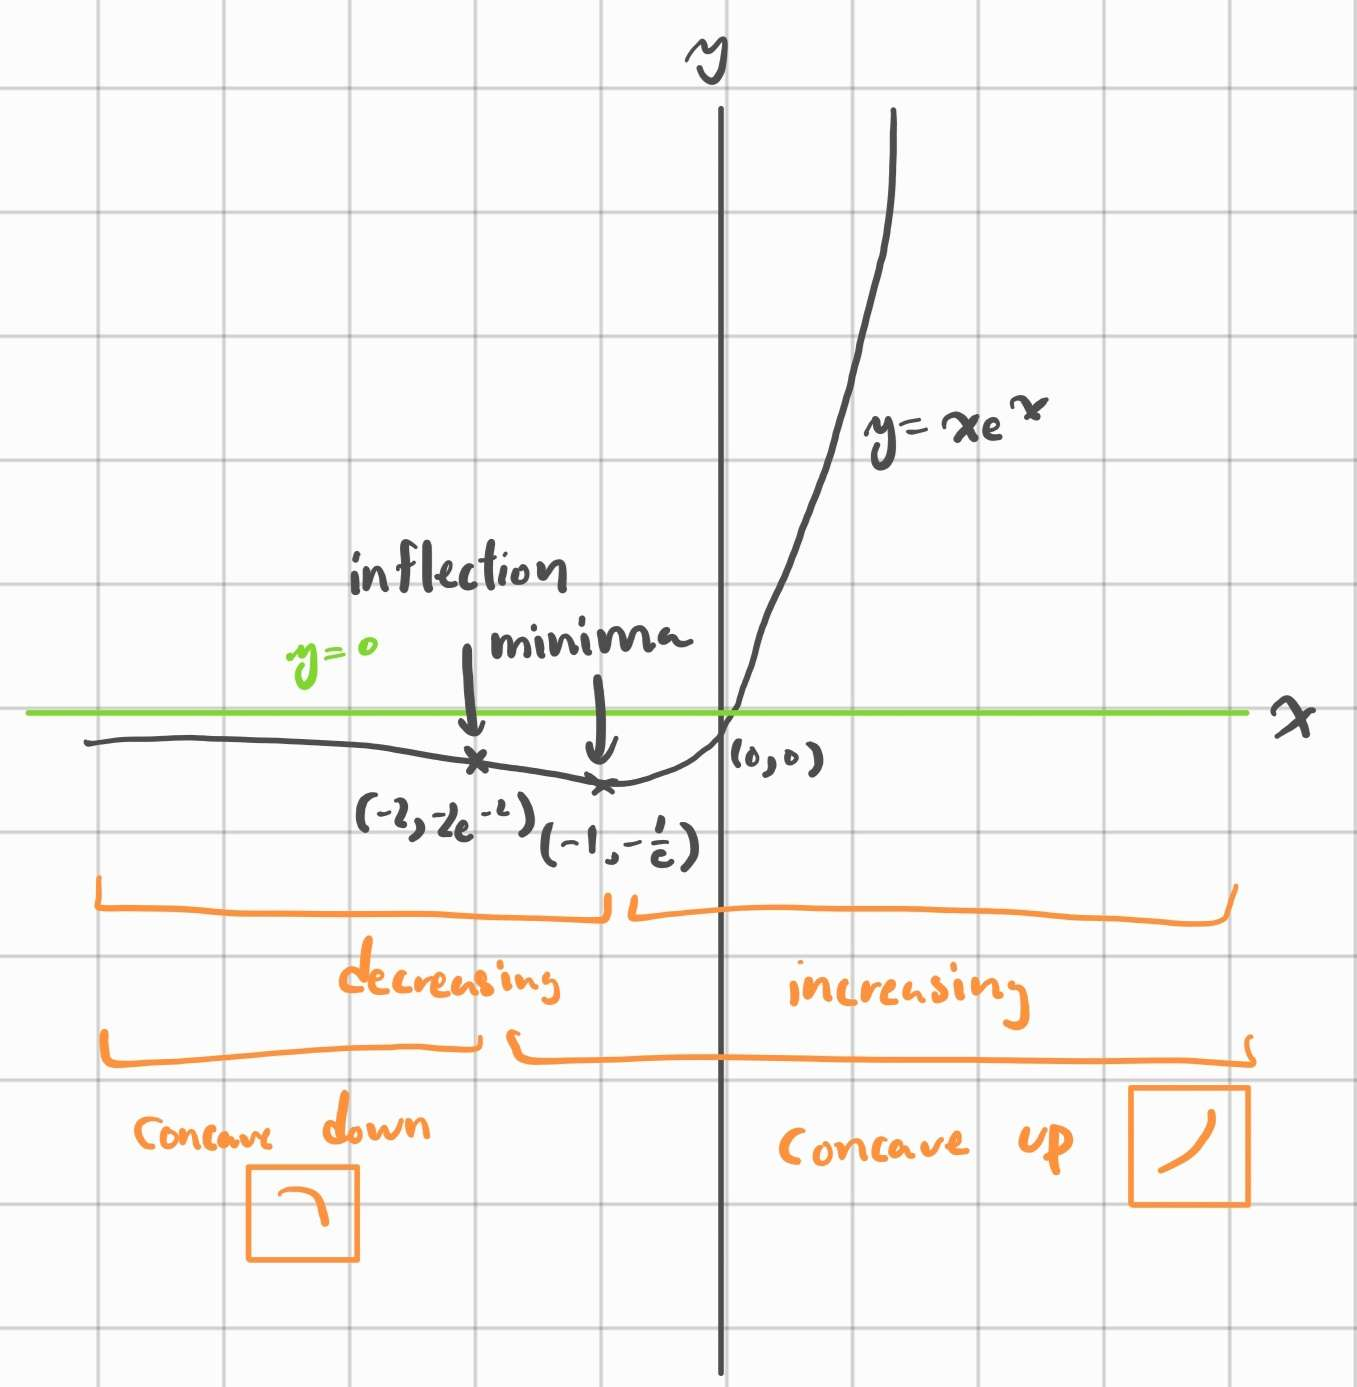
\includegraphics[width=\textwidth]{A2Q8.jpg}
\end{minipage}

\end{document}